\documentclass[11pt]{article}
\usepackage[margin=20mm]{geometry}
\usepackage{amsmath}
\usepackage{listings,color,enumitem}
\definecolor{mygreen}{RGB}{28,172,0} % color values Red, Green, Blue
\definecolor{mylilas}{RGB}{170,55,241}
\usepackage{graphicx}
\title{Problem Set 1\\ \vspace{2mm}\Large{16-642 Manipulation, Estimation, and Control}}
\author{Matthew Swenson}

\begin{document}
	\maketitle
	
\section{Question 1}
\begin{enumerate}[label=\Alph*]
    \item 4
    \item 1
    \item 6
    \item 1
    \item $\infty$, because the trunk is being modeled as an infinitely variable curve. However, in real life the DOF of an elephant trunk is probably somewhere between 6-8, due to the limited number of major muscle groups in the trunk (the internet varies in the actual number). 
\end{enumerate}
\section{Question 2}
We know $H^0_1 H^1_0 = I$. Therefore, we can write: 
$$
\begin{bmatrix}
    R^0_1  & d^0_1  \\
    \vec{0} & 1
\end{bmatrix}
\begin{bmatrix}
    R^"& & d^"  \\
    \vec{0} & 1
\end{bmatrix}
=
I
$$
$$
\begin{bmatrix}
    R^0_1R^"& R^0_1d^"+d^0_1  \\
    \vec{0} & 1
\end{bmatrix}
\begin{bmatrix}
    R^0_1& & d^0_1  \\
    \vec{0} & 1
\end{bmatrix}
=
I
$$
We can then break this into two separate equations and solve them seprately: 
\begin{align*}
R^0_1R^" = I 
&&
R^0_1d^"+d^0_1  = 0 
\\
R^" = \big[R^0_1\big]^T 
&& 
d^"= -\big[R^0_1\big]^T  d^0_1  
\end{align*}
Therefore,
$$
H^1_0 =
\begin{bmatrix}
    \big[R^0_1\big]^{ T} & -\big[R^0_1\big]^{T } d^0_1  \\
    \vec{0}& 1
\end{bmatrix}
$$
\section{Question 3}
$$
H^1_0 = Trans_{y,5}Trans_{z,6}Rot_{x,90}Rot_{z,-60}
$$
$$
H^1_0 =
\begin{bmatrix}
    1 & 0 & 0 & 0 \\
    0 & 1 & 0 & 5 \\
    0 & 0 & 1 & 6 \\
    0 & 0 & 0 & 1 \\
\end{bmatrix}
\begin{bmatrix}
    1 & 0 & 0 & 0 \\
    0 & 0 & -1& 0 \\
    0 & 1 & 0 & 0 \\
    0 & 0 & 0 & 1 \\
\end{bmatrix}      
\begin{bmatrix}
    \frac{1}{2} & \frac{\sqrt{3}}{2} & 0 & 0 \\
    -\frac{\sqrt{3}}{2}  & \frac{1}{2} & 0 & 0 \\
    0 & 0 & 1 & 0 \\
    0 & 0 & 0 & 1 \\
\end{bmatrix}
=
\begin{bmatrix}
    \frac{1}{2} & \frac{\sqrt{3}}{2} & 0 & 0 \\
    0 & 0 & -1 & 5 \\
    -\frac{\sqrt{3}}{2}  & \frac{1}{2} & 0 & 6 \\
    0 & 0 & 0 & 1 \\
\end{bmatrix}
$$
\section{Question 4}
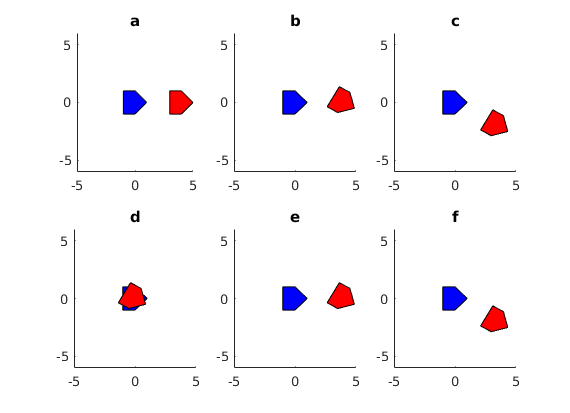
\includegraphics{p4.png}
\section{Question 5}
We can write the transformaiton for the screw to the base frame as 
$$
H^b_s = H^b_c H^c_s 
$$
And we can write the transformaiton for the screwdriver tip to the base frame as 
$$
H^b_t = H^b_w H^w_t 
$$
Because we want the transformation of $H^b_w$ when the screwdriver tip and screw are colocated,
we can write
$$
 H^b_w H^w_t  =H^b_c H^c_s  
$$
$$
H^b_w =
H^b_c H^c_s \big[H^w_t \big]^{-1 }
$$
\section{Question 6}
$$
H^{Pittsburgh}_{Greenwhich} = 
H_{Pittsburgh_z}^{Pittsburgh} 
H_{Pittsburgh_y}^{Pittsburgh_z} 
H_{Center}^{Pittsburgh_y} 
H^{Center}_{Greenwhich_y}
H^{Greenwhich_y}_{Greenwhich} 
$$
\begin{align*}
H_{P_z}^P = 
\begin{bmatrix}
    1 & 0 & 0 & 0 \\
    0 & 1 & 0 & 0 \\
    0 & 0 & 1 & 6000 \\
    0 & 0 & 0 & 1 \\
\end{bmatrix}
&&
H^{P_z}_{P_y} =
\begin{bmatrix}
    \cos{40.5} & 0 & -\sin{40.5} & 0 \\
    0&  1 & 0 & 0 \\
    \sin{40.5} &0&\cos{40.5} & 0 \\
    0& 0 & 0 & 1 \\
\end{bmatrix}
&&
H^{P_y}_{C} =
\begin{bmatrix}
    1 & 0 & 0 & 0 \\
    0 & \cos{80} & -\sin{80} & 0 \\
    0 & \sin{80} &\cos{80} & 0 \\
    0 & 0 & 0 & 1 \\
\end{bmatrix}
\end{align*}
\begin{align*}
H_{G_y}^{C} =
\begin{bmatrix}
    \cos{-51} & 0 & \sin{-51} & 0 \\
    0&  1 & 0 & 0 \\
    -\sin{-51} &0&\cos{-51} & 6000 \\
    0& 0 & 0 & 1 \\
\end{bmatrix}
&&
H_{P_z}^P = 
\begin{bmatrix}
    1 & 0 & 0 & 0 \\
    0 & 1 & 0 & 0 \\
    0 & 0 & 1 & -6000 \\
    0 & 0 & 0 & 1 \\
\end{bmatrix}
\end{align*}

$$
H_{Greenwhich}^Pittsburgh = 
\begin{bmatrix}
    0.56618  &0.63958  & -0.51997 &    3119.8  \\
    -0.76534  &0.17365 &  -0.61976&     3718.6 \\
    -0.30609  &0.74885 &   0.58781&     2473.1 \\
           0  &      0 &         0&          1 \\
\end{bmatrix}
$$


\section{Question 7}
We know $p' = Rp$ and $p' = QPQ^*$, where $Q^*=[q_0,-q_1,-q_2,-q_3]^T$ and $P=[0,p_1,p_2,p_3]^T$\\
Therefore, $Rp = QPQ^*$
The Hamiltonian product of two quaternions is 
$$
(q_1,q_2,q_3,q_4)(p_1,p_2,p_3,p_4)=\left(\begin{array}{c} p_{1}\,q_{1}-p_{2}\,q_{2}-p_{3}\,q_{3}-p_{4}\,q_{4}\\ p_{1}\,q_{2}+p_{2}\,q_{1}+p_{3}\,q_{4}-p_{4}\,q_{3}\\ p_{1}\,q_{3}+p_{3}\,q_{1}-p_{2}\,q_{4}+p_{4}\,q_{2}\\ p_{1}\,q_{4}+p_{2}\,q_{3}-p_{3}\,q_{2}+p_{4}\,q_{1} \end{array}\right)
$$
For our specific P and Q, this becomes:
$$
QP=\left(\begin{array}{c} -p_{1}\,q_{1}-p_{2}\,q_{2}-p_{3}\,q_{3}\\ p_{1}\,q_{0}-p_{2}\,q_{3}+p_{3}\,q_{2}\\ p_{2}\,q_{0}+p_{1}\,q_{3}-p_{3}\,q_{1}\\ p_{2}\,q_{1}-p_{1}\,q_{2}+p_{3}\,q_{0} \end{array}\right)
$$
This is also a quaternion, so:
\begin{align*}
Q&PQ^*=\\
      &\left(\begin{array}{c} q_{1}\,\left(p_{1}\,q_{0}-p_{2}\,q_{3}+p_{3}\,q_{2}\right)-q_{0}\,\left(p_{1}\,q_{1}+p_{2}\,q_{2}+p_{3}\,q_{3}\right)+q_{2}\,\left(p_{2}\,q_{0}+p_{1}\,q_{3}-p_{3}\,q_{1}\right)+q_{3}\,\left(p_{2}\,q_{1}-p_{1}\,q_{2}+p_{3}\,q_{0}\right)\\ q_{0}\,\left(p_{1}\,q_{0}-p_{2}\,q_{3}+p_{3}\,q_{2}\right)+q_{2}\,\left(p_{2}\,q_{1}-p_{1}\,q_{2}+p_{3}\,q_{0}\right)+q_{1}\,\left(p_{1}\,q_{1}+p_{2}\,q_{2}+p_{3}\,q_{3}\right)-q_{3}\,\left(p_{2}\,q_{0}+p_{1}\,q_{3}-p_{3}\,q_{1}\right)\\ q_{0}\,\left(p_{2}\,q_{0}+p_{1}\,q_{3}-p_{3}\,q_{1}\right)-q_{1}\,\left(p_{2}\,q_{1}-p_{1}\,q_{2}+p_{3}\,q_{0}\right)+q_{2}\,\left(p_{1}\,q_{1}+p_{2}\,q_{2}+p_{3}\,q_{3}\right)+q_{3}\,\left(p_{1}\,q_{0}-p_{2}\,q_{3}+p_{3}\,q_{2}\right)\\ q_{0}\,\left(p_{2}\,q_{1}-p_{1}\,q_{2}+p_{3}\,q_{0}\right)+q_{1}\,\left(p_{2}\,q_{0}+p_{1}\,q_{3}-p_{3}\,q_{1}\right)-q_{2}\,\left(p_{1}\,q_{0}-p_{2}\,q_{3}+p_{3}\,q_{2}\right)+q_{3}\,\left(p_{1}\,q_{1}+p_{2}\,q_{2}+p_{3}\,q_{3}\right) \end{array}\right) \\
Q&PQ^*=\left(\begin{array}{c} 0\\ p_{1}\,{q_{0}}^2+2\,p_{3}\,q_{0}\,q_{2}-2\,p_{2}\,q_{0}\,q_{3}+p_{1}\,{q_{1}}^2+2\,p_{2}\,q_{1}\,q_{2}+2\,p_{3}\,q_{1}\,q_{3}-p_{1}\,{q_{2}}^2-p_{1}\,{q_{3}}^2\\ p_{2}\,{q_{0}}^2-2\,p_{3}\,q_{0}\,q_{1}+2\,p_{1}\,q_{0}\,q_{3}-p_{2}\,{q_{1}}^2+2\,p_{1}\,q_{1}\,q_{2}+p_{2}\,{q_{2}}^2+2\,p_{3}\,q_{2}\,q_{3}-p_{2}\,{q_{3}}^2\\ p_{3}\,{q_{0}}^2+2\,p_{2}\,q_{0}\,q_{1}-2\,p_{1}\,q_{0}\,q_{2}-p_{3}\,{q_{1}}^2+2\,p_{1}\,q_{1}\,q_{3}-p_{3}\,{q_{2}}^2+2\,p_{2}\,q_{2}\,q_{3}+p_{3}\,{q_{3}}^2 \end{array}\right) \\
Q&PQ^*=\left(\begin{array}{c} 0\\ \left({q_{0}}^2+{q_{1}}^2-{q_{2}}^2-{q_{3}}^2\right)\,p_{1}+\left(2\,q_{1}\,q_{2}-2\,q_{0}\,q_{3}\right)\,p_{2}+\left(2\,q_{0}\,q_{2}+2\,q_{1}\,q_{3}\right)\,p_{3}\\ \left(2\,q_{0}\,q_{3}+2\,q_{1}\,q_{2}\right)\,p_{1}+\left({q_{0}}^2-{q_{1}}^2+{q_{2}}^2-{q_{3}}^2\right)\,p_{2}+\left(2\,q_{2}\,q_{3}-2\,q_{0}\,q_{1}\right)\,p_{3}\\ \left(2\,q_{1}\,q_{3}-2\,q_{0}\,q_{2}\right)\,p_{1}+\left(2\,q_{0}\,q_{1}+2\,q_{2}\,q_{3}\right)\,p_{2}+\left({q_{0}}^2-{q_{1}}^2-{q_{2}}^2+{q_{3}}^2\right)\,p_{3} \end{array}\right) \\
\end{align*}
From this last form, we can see that the bottom three entries in the vector have a 
very similar form to a 3x3 matrix multiplied by $[p1,p2,p3]^T$. Discarding the 0 and pulling out $p$, we get
$$
R = 
\begin{bmatrix}
{q_{0}}^2+{q_{1}}^2-{q_{2}}^2-{q_{3}}^2 & 2\,q_{1}\,q_{2}-2\,q_{0}\,q_{3}         & 2\,q_{0}\,q_{2}+2\,q_{1}\,q_{3}\\
2\,q_{0}\,q_{3}+2\,q_{1}\,q_{2}         & {q_{0}}^2-{q_{1}}^2+{q_{2}}^2-{q_{3}}^2 & 2\,q_{2}\,q_{3}-2\,q_{0}\,q_{1}\\
2\,q_{1}\,q_{3}-2\,q_{0}\,q_{2}         & 2\,q_{0}\,q_{1}+2\,q_{2}\,q_{3}         & {q_{0}}^2-{q_{1}}^2-{q_{2}}^2+{q_{3}}^2
\end{bmatrix} 
$$
\section{Question 8}
$$
R_0^1=
\begin{bmatrix}
    \cos{\theta_1} & -\sin{\theta_1} & 0 \\
    \sin{\theta_1} &\cos{\theta_1} & 0 \\
    0    & 0 & 1 \\
\end{bmatrix}
\begin{bmatrix}
    \cos{\theta_2} & 0 & \sin{\theta_2} \\
    0    & 1 & 0 \\
    -\sin{\theta_2} & 0 &\cos{\theta_2} \\
\end{bmatrix}
\begin{bmatrix}
    \cos{\theta_3} & -\sin{\theta_3} & 0 \\
    \sin{\theta_3} &\cos{\theta_3} & 0 \\
    0    & 0 & 1 \\
\end{bmatrix}
$$

This arrangement of linkages results in a rotation matrix similar to a XYX euler angle rotation. 

\end{document}
